\documentclass[12pt]{article}

\usepackage[letterpaper,margin=2.5cm]{geometry}
\usepackage{times}
\usepackage[T1]{fontenc}
\usepackage[english]{babel}
\usepackage{microtype}
\usepackage{graphicx}
\usepackage{booktabs}
\usepackage{amsmath,amssymb}
\usepackage{authblk}
\PassOptionsToPackage{hyphens}{url}
\usepackage[colorlinks=true,citecolor=blue,linkcolor=blue,urlcolor=blue,breaklinks=true]{hyperref}
\usepackage[round]{natbib}
\usepackage{setspace}
\usepackage{caption}
\usepackage{enumitem}
\usepackage[right]{lineno}
\usepackage{ragged2e}

\setcitestyle{numbers,square}
\setlength{\bibsep}{4pt}
\onehalfspacing

\title{\Large Zero-Shot Vision-Language Models versus LoRA-Fine-Tuned TrOCR for Handwritten Medical Prescription Recognition: A Benchmark and Clinical Safety-Aware Error Analysis}

% PLACEHOLDER --- confirm real name / affiliation / ORCID before submission.
\author[1]{Bang Dang}
\affil[1]{Independent Researcher}
\renewcommand\Authands{ and }

\date{}

\begin{document}

\linenumbers
\RaggedRight

\maketitle

\begin{center}
\textit{Corresponding author: Bang Dang (\href{mailto:bangdang007112@gmail.com}{bangdang007112@gmail.com})}\\[2pt]
\textit{Target venue: PeerJ Computer Science (AI Application track)}
\end{center}

% Note to author, remove before submission: confirm the name/affiliation string above and add an ORCID
% if available. (Moved out of the rendered PDF -- it was previously visible body text inside a \quote block.)

\begin{abstract}
Handwritten prescriptions are a recognized source of medication error, which makes automatic transcription
a natural application for optical character recognition (OCR). Recent general-purpose vision-language
models (VLMs) are often described as strong OCR systems, but none has been systematically benchmarked on
public handwritten-prescription data or compared against a fine-tuned OCR specialist under matched
conditions. We benchmark seven systems zero-shot --- Tesseract, EasyOCR, TrOCR-large-handwritten, Donut,
GOT-OCR2.0, Qwen2.5-VL-3B-Instruct, and PaddleOCR-VL, the last of which we were ultimately unable to run due
to an unresolved upstream library conflict --- on a public Bangladeshi handwritten-prescription dataset
(78 drug classes, 780 held-out images) and on IAM (400 images) as an out-of-domain control. The strongest
zero-shot system on the prescription domain is a 3-billion-parameter general VLM, Qwen2.5-VL-3B
(character error rate, CER, of 0.434), ahead of every dedicated OCR model we tested. We then fine-tune
TrOCR-large-handwritten (558M parameters) with Low-Rank Adaptation (LoRA) on 3{,}120 training images,
running a rank ablation (r = 8, 16, 32) and an augmentation ablation before settling on r = 32. The
fine-tuned model reaches a CER of 0.114 on the prescription test set --- an 80.3\% relative reduction from
zero-shot --- and is significantly better than every zero-shot system tested, including Qwen2.5-VL-3B
(Wilcoxon signed-rank, $p = 4.4\times10^{-59}$) and GOT-OCR2.0 ($p = 8.0\times10^{-93}$), despite touching
under 2\% of the model's parameters and running on a single free-tier GPU. On IAM, the same model's CER
rises from 0.441 to 0.501 ($p = 3.2\times10^{-4}$), a real but partial loss of general handwriting ability.
Looking at error categories rather than aggregate CER, fine-tuning cuts outright nonsensical output
by roughly four-fold, but the errors that remain shift toward predictions that read as a \textit{different,
real} drug name --- a smaller category, but arguably the more dangerous one, since it is far less likely to
be caught on manual review than an obviously wrong transcription. We saw no meaningful sign of a related
risk, namely the model inserting memorized drug names into ordinary text it had never been trained on. Code,
frozen evaluation data, and the trained adapter are released to support exact reproduction on free-tier
cloud GPUs.

\vspace{4pt}
\noindent\textbf{Keywords:} optical character recognition, handwritten text recognition, vision-language
models, LoRA, parameter-efficient fine-tuning, catastrophic forgetting, medication safety, clinical NLP
\end{abstract}

\section{Introduction}

Illegible or misread handwriting on prescriptions is a well-documented contributor to medication error
\citep{Bryan2021LASA,Ostini2012LASA}, which makes automatic reading of handwritten prescriptions more than
a convenience: done well, it could flag ambiguous entries before they ever reach a pharmacy counter.
Handwritten text recognition (HTR), the underlying technical problem, has gone through several distinct
generations of approach. Early systems relied on binarization and template matching. These gave way to
CNN--RNN sequence models trained with connectionist temporal classification loss, of which Tesseract's
LSTM-based engine \citep{Smith2007Tesseract} is a widely deployed example. TrOCR \citep{Li2023TrOCR} recast
recognition as sequence-to-sequence translation, pairing a vision transformer encoder with an autoregressive
text decoder. Donut \citep{Kim2022Donut} went further and dropped explicit character-level modeling
altogether, training an image-to-text transformer end to end on synthetic full-page documents. Most
recently, general-purpose vision-language models --- GOT-OCR2.0 \citep{Wei2024GOTOCR},
Qwen2.5-VL \citep{Bai2025Qwen}, PaddleOCR-VL \citep{Cui2025PaddleOCRVL} --- have started to treat OCR as one
capability among many rather than a dedicated training objective.

That diversification leaves a fairly ordinary practical question unanswered: for someone actually building
a prescription-reading system today, which of these approaches works, and is it worth fine-tuning a smaller
specialist model rather than simply prompting a large general VLM? We are not aware of a published study
that benchmarks this particular mix --- classical OCR, specialist HTR transformers, an OCR-free document
model, and current-generation general VLMs --- on a \textit{public} prescription dataset, let alone couples
that benchmark with a lightweight fine-tuning step and an explicit check of how much general handwriting
ability it costs.

This paper makes five contributions:

\begin{enumerate}[leftmargin=*]
\item A zero-shot benchmark of seven OCR/VLM systems on a public handwritten-prescription dataset (the
Kaggle ``Doctor's Handwritten Prescription BD dataset'' \citep{Mia2024KaggleRx}) and on
IAM \citep{Marti2002IAM} as an out-of-domain control, reported with bootstrap confidence intervals and, for
model pairs scored on identical frozen test images, paired Wilcoxon signed-rank tests.
\item Evidence that LoRA-adapting \citep{Hu2022LoRA} a 558M-parameter specialist model, updating under 2\%
of its parameters on one free-tier GPU, statistically outperforms every zero-shot system we tried on the
target domain, including a 3B-parameter general VLM and a purpose-built ``OCR-2.0'' model of roughly
comparable size.
\item A full rank (r = 8/16/32) and augmentation ablation showing that a commonly used default rank, 16,
was in fact beaten on both axes we measured --- in-domain accuracy and out-of-domain retention --- by a
higher rank, 32. We take this as a caution against treating a LoRA rank choice as safe simply because it is
common practice.
\item A statistically grounded look at catastrophic forgetting under LoRA: fine-tuning measurably
\textit{hurts} performance on out-of-domain handwriting, even at under 2\% of parameters touched, which
complicates any simple reading of prior work suggesting LoRA is largely protective against
forgetting \citep{Biderman2024LoRALearnsLess}.
\item What we believe is the first analysis linking OCR error \textit{type}, rather than raw error rate, to
medication-name-confusion risk: after fine-tuning, nonsensical output drops sharply, but the errors that
remain skew toward predictions that resemble a different real drug name --- exactly the category standard
CER reporting is blind to.
\end{enumerate}

Section~2 reviews related work; Section~3 describes the datasets, models, and evaluation and fine-tuning
protocol; Section~4 reports results; Section~5 discusses their implications and positions this work against
the closest prior study; Section~6 states limitations; Section~7 concludes.

\section{Related Work}

\subsection{Handwritten text recognition, from sequence models to transformers}

Classical HTR pipelines pair explicit segmentation with CNN/RNN recognizers trained under CTC loss; Tesseract's
LSTM engine \citep{Smith2007Tesseract} remains a common baseline of this family. TrOCR \citep{Li2023TrOCR}
reframed recognition as translation, combining a vision transformer encoder with an autoregressive decoder
and pretraining on large synthetic corpora before fine-tuning on handwriting benchmarks such as IAM. Donut
\citep{Kim2022Donut} removed the recognition step as a distinct stage, training end to end on synthetic
document images (SynthDoG). As Section~4.1 shows, that choice of pretraining data makes Donut largely
unusable, absent further fine-tuning, on isolated handwritten words: its training distribution assumes
full-page layouts that a single cropped word simply does not have. Two recent surveys
\citep{GarridoMunoz2026Survey,AlKendi2024Survey} cover this progression in more depth than we have room for
here.

\subsection{General-purpose vision-language models as OCR systems}

A separate and more recent line of work treats OCR as one of several capabilities in a large VLM rather
than the model's reason for existing. GOT-OCR2.0 \citep{Wei2024GOTOCR} targets a broad ``OCR-2.0''
definition spanning text, formulas, charts, and tables, but is released and updated largely outside the
standard \texttt{transformers} library's normal release cadence, which, as we detail in Sections~4 and 5.6,
leaves it unusually sensitive to version drift. Qwen2.5-VL \citep{Bai2025Qwen} and
PaddleOCR-VL \citep{Cui2025PaddleOCRVL} are general-purpose or document-parsing-oriented VLMs for which text
recognition is emergent rather than dedicated. Crosilla et al.\ \citep{Crosilla2025LLMHTR} recently
benchmarked several such general multimodal models against task-specific HTR systems and found a pattern
broadly similar to ours: general models are competitive zero-shot but not uniformly better, and evaluation
is complicated by non-OCR behavior --- refusals, hedged answers --- that ordinary error metrics were not
designed to anticipate. We run into exactly this problem with Qwen2.5-VL on IAM (Section~4.1).

\subsection{Parameter-efficient fine-tuning and forgetting}

LoRA \citep{Hu2022LoRA} fine-tunes a frozen pretrained model by learning a pair of low-rank update matrices
for each targeted weight, so that only a small fraction of parameters is ever updated. Chang and
Li \citep{ChangLi2024DLoRA} apply a related decomposition to TrOCR (DoRA on the encoder, LoRA on the
decoder), reporting 4.02\% CER on IAM while touching roughly 0.7\% of parameters --- the closest prior
demonstration that LoRA-family methods work for TrOCR specifically, though without a
fine-tuning-domain-versus-generalization comparison. Whether PEFT methods actually reduce catastrophic
forgetting relative to full fine-tuning is still unsettled. Biderman et al.\
\citep{Biderman2024LoRALearnsLess} argue that LoRA forgets less than full fine-tuning under matched
performance; Shuttleworth et al.\ \citep{Shuttleworth2025Illusion} show LoRA-tuned weights develop
structurally distinct ``intruder dimensions'' that offer a mechanistic account of why LoRA solutions can
behave differently from full fine-tuning even at comparable in-domain accuracy; and Kalajdzievski
\citep{Kalajdzievski2024Scaling} reports that forgetting under fine-tuning follows a fairly predictable
scaling law and is not reliably avoided by early stopping alone. Our results (Section~4.4) add a concrete,
statistically tested data point to this question in a domain --- handwriting recognition --- where it has
not, to our knowledge, been examined before: LoRA at both r = 16 and r = 32 produces a significant, though
partial, degradation on out-of-domain data, which sits closer to Shuttleworth et al.'s and Kalajdzievski's
framing than to an unqualified reading of ``LoRA forgets less.''

\subsection{Prior work on prescription and medical handwriting OCR}

The dataset we use, the Kaggle ``Doctor's Handwritten Prescription BD dataset,'' comes from Mia et
al.\ \citep{Mia2024KaggleRx}, who trained a VGG16 classifier on it. Ali et al.\
\citep{Ali2024Prescription} fine-tune a Mask R-CNN segmentation stage together with TrOCR-Base-Handwritten
on roughly 1{,}000 handwritten Pakistani prescriptions (augmented tenfold), reporting CER between 1.4\% and
15.4\% depending on the test scenario --- the closest prior demonstration that fine-tuning a TrOCR-family
model works at prescription scale, though on a different, private dataset and without a
forgetting analysis. A hybrid
Tesseract/PaddleOCR/GPT-4o pipeline for prescription reading has also been
reported \citep{FrontiersMed2026Hybrid}, using a different model lineup and web-scraped rather than
benchmark-standard data. Cheema et al.\ \citep{Cheema2024PeerJUrdu} published a related methodological
precedent --- adapting multilingual VLMs, with TrOCR as one comparison point, for low-resource Urdu OCR ---
in \textit{PeerJ Computer Science}, the venue we target here.

\subsection{Medication-name confusion as a patient-safety problem}

Separately from OCR, the clinical pharmacy literature has long treated structurally or phonetically similar
drug names --- ``look-alike, sound-alike'' (LASA) pairs --- as a distinct and well-studied source of
medication error \citep{Bryan2021LASA,Ostini2012LASA,LizanoDiez2020LASA}. Karet \citep{Karet2023TallMan}
quantifies orthographic and phonetic similarity across FDA/ISMP-flagged LASA pairs, which gives us a
methodological precedent for treating ``resembles a different real drug'' as a distinct, measurable error
category rather than folding it into an undifferentiated error rate, the approach we adopt in
Sections~3.5 and 4.5. The closest analogue we found for connecting error \textit{type}, rather than raw
rate, to clinical risk in an automated-transcription setting is Zhou et al.\ \citep{Zhou2018JAMA}, who
classify speech-recognition errors in clinical dictation by clinical significance. We are not aware of prior
work making this connection for OCR-based prescription reading specifically, which is the gap our
error-taxonomy analysis (Section~4.5) tries to fill.

\section{Materials and Methods}

Code, frozen evaluation manifests, per-image predictions, and the final LoRA adapter are released alongside
this paper (see Data Availability) so the results below can be reproduced exactly.

\subsection{Datasets}

\textbf{Kaggle-Rx.} The ``Doctor's Handwritten Prescription BD dataset'' \citep{Mia2024KaggleRx}
(\url{mamun1113/doctors-handwritten-prescription-bd-dataset} on Kaggle) contains cropped, single-word
handwritten images of 78 drug names, pre-split by the dataset authors into \texttt{Training},
\texttt{Validation}, and \texttt{Testing} folders with accompanying label files. We verified the actual
split sizes by direct enumeration rather than trusting the dataset page's summary description, which states
an approximate 60/20/20 split that does not match the file counts we observe: the real split is
\textbf{Training = 3{,}120, Validation = 780, Testing = 780} images (4{,}680 total), all of which resolve
correctly against their labels. We hold out the entire \texttt{Testing} split as a frozen evaluation set,
used identically, down to the image-filename level, for every zero-shot model and for the fine-tuned
model's final evaluation. We confirmed this manifest returns the same 780 images across seven independent
runs (fixed seed = 42) before relying on it for paired statistical tests.

\textbf{IAM.} We use the IAM Handwriting Word Database \citep{Marti2002IAM} as an out-of-domain control
representing general, non-medical English handwriting, drawing a fixed random subsample of 400 word images
(seed = 42, again verified identical across runs) through the Kaggle mirror
\url{nibinv23/iam-handwriting-word-database}. IAM serves two purposes here: a domain-shift baseline
against which to read Kaggle-Rx performance, and a generalization probe for the fine-tuned model, which
never sees IAM during training.

\subsection{Models evaluated zero-shot}

{\small
We group seven systems into three families. \textit{Classical}: Tesseract \citep{Smith2007Tesseract}
(LSTM-based engine) and EasyOCR (CRAFT detector with a CRNN recognizer, used here in single-word mode).
\textit{Specialist encoder-decoder / document-understanding transformers}:
\texttt{microsoft/trocr-large-handwritten} \citep{Li2023TrOCR} (558M parameters) and
\texttt{naver-clova-ix/donut-base} \citep{Kim2022Donut}, the latter tested both on raw word crops and on
crops padded onto a blank page-sized canvas to better match its SynthDoG pretraining aspect ratio.
\textit{General-purpose vision-language models}: \texttt{stepfun-ai/GOT-OCR-2.0-hf} \citep{Wei2024GOTOCR}
(roughly 580M parameters), \texttt{Qwen/Qwen2.5-VL-3B-Instruct} \citep{Bai2025Qwen} (3B parameters, prompted
with a fixed instruction to output only the transcribed text), and
\texttt{PaddlePaddle/PaddleOCR-VL} \citep{Cui2025PaddleOCRVL} (0.9B parameters). The last of these is
included in our pipeline but excluded from the results we report: it raises a \texttt{TypeError} inside its
own \texttt{trust\_remote\_code} modeling file (\texttt{create\_causal\_mask() got an unexpected keyword
argument `inputs\_embeds'}) under every \texttt{transformers} version we tried, matching an open, unresolved
community bug report of the same problem. We treat this as a reproducibility finding worth reporting in its
own right (Section~5.6) rather than a gap to quietly leave out.
\par}

Every zero-shot model was first run on five images and checked for non-degenerate output before we
committed to the full 1{,}180-image (780 + 400) evaluation, and \texttt{transformers==4.57.0} was pinned
after an initial run with an unpinned, newly released major version produced incoherent output for
GOT-OCR2.0 (Section~5.6) --- a library-version sensitivity worth flagging for anyone benchmarking this class
of model.

\subsection{Evaluation protocol}

For every (model, image) pair we compute:

\begin{itemize}[leftmargin=*]
\item \textbf{Character error rate (CER)} and \textbf{word error rate (WER)}, via Levenshtein edit distance
(case-insensitive, whitespace-normalized), using \texttt{rapidfuzz} and \texttt{jiwer} respectively.
\item \textbf{Exact match}, string equality after the same normalization.
\item \textbf{Closed-vocabulary top-1 accuracy} (Kaggle-Rx only): the raw prediction is mapped to its
nearest of the 78 drug names by minimum normalized edit distance, and that label is compared to ground
truth. This captures cases where free-text output is close enough to be resolved unambiguously against a
known drug list, which is arguably closer to how such a system would be used in practice --- checked against
a pharmacy formulary --- than raw string matching is.
\item \textbf{A degenerate-output flag}: empty output, output over 200 characters, or a short token repeated
so that fewer than one-sixth of tokens are unique. This separates ``the model broke'' from ``the model gave
a fluent but wrong answer,'' a distinction we needed after seeing near-100\% of Donut's raw-crop outputs
fall into the former category (Section~4.1).
\end{itemize}

We report the mean and 95\% bootstrap confidence interval (1{,}000 resamples, fixed seed = 0) for CER, and,
wherever two models were scored on the same frozen image set, a paired Wilcoxon signed-rank test on
per-image CER. This pairing is valid here specifically because every model's evaluation manifest comes from
the same seeded procedure and was checked to return an identical image set across independent runs. Where a
model's CER distribution turns out to be heavily right-skewed (Section~4.1), we report the median alongside
the mean.

For every paired comparison we additionally report the matched-pairs rank-biserial correlation as an effect
size, $r = (W_{+} - W_{-}) / (W_{+} + W_{-})$, computed directly from the signed ranks of the non-zero
differences rather than back-derived from the test statistic; it is bounded in $[-1, 1]$, with its sign
following (model A $-$ model B) \citep{Cureton1956RankBiserial}. Wilcoxon signed-rank on per-image CER is the
field-standard choice for paired system comparisons of this kind \citep{Dror2018Wilcoxon}. Because we run
multiple paired comparisons, we apply Holm--Bonferroni correction \citep{Holm1979} \textit{within} two
pre-specified families -- cross-model benchmark comparisons (Sections~4.1, 4.3, 4.4; seven comparisons) and
within-method rank/augmentation ablation comparisons (Section~4.2; six comparisons) -- rather than across
all thirteen comparisons jointly, since the two families answer different questions and pooling them would
over-correct the family a reader actually cares about; both families and the exact test order were fixed
before inspecting any $p$-value. We follow Dem\v{s}ar's \citep{Demsar2006} recommendation of Holm's
step-down procedure over plain Bonferroni, since it is uniformly more powerful and requires no additional
independence assumption. The script implementing this (\texttt{src/analyze\_statistics.py}) is released
alongside the paper (Data Availability).

\subsection{LoRA fine-tuning of TrOCR-large-handwritten}

We fine-tune \texttt{microsoft/trocr-large-handwritten} with LoRA (via the \texttt{peft} library), targeting
the attention projections of both the encoder (\texttt{query}, \texttt{value}) and decoder
(\texttt{q\_proj}, \texttt{v\_proj}), with dropout 0.1 and no bias adaptation. Training uses the full
3{,}120-image \texttt{Training} split with an Albumentations augmentation pipeline --- affine
rotation/shear/scale, elastic distortion, Gaussian noise and blur, brightness/contrast jitter, morphological
erosion/dilation --- a 300-image random subsample of \texttt{Validation} for epoch-level tracking, AdamW
with a cosine schedule (peak learning rate $2\times10^{-4}$, 8--10\% warmup), an effective batch size of 16
(8 physical $\times$ 2 gradient-accumulation steps) under \texttt{fp16} mixed precision (\texttt{bf16} is
not well supported on the Turing-architecture T4 GPUs used here), up to 15 epochs with early stopping
(patience of 5 epochs on validation CER), and a five-hour wall-clock cutoff per run. Training runs on a
single Kaggle Notebooks session (Kaggle's standard GPU-enabled, Ubuntu-based Python Docker image) with two
NVIDIA T4 GPUs (16GB each) under automatic \texttt{DataParallel}, using \texttt{transformers==4.57.0}
(pinned; see Section~3.2), \texttt{peft} for the LoRA implementation, and \texttt{torchao>=0.16.0} (the
Kaggle base image's default \texttt{torchao==0.10.0} is incompatible with \texttt{peft}'s
\texttt{get\_peft\_model} and must be upgraded explicitly).

\textbf{Rank and augmentation ablation.} Rather than fixing the LoRA rank in advance, we trained to early
stopping for three ranks (r $\in \{8, 16, 32\}$, $\alpha = 2r$ throughout, elastic distortion on) and, with
rank held at 16, for augmentation on versus off, evaluating all four resulting checkpoints on the same
frozen Kaggle-Rx and IAM test sets described above. We picked the configuration reported as ``the'' fine-tuned
model by frozen-test CER on both datasets jointly, rather than committing to a rank beforehand, precisely
because the ablation is what tells us which configuration to report as primary (Section~4.2). One caveat we
want to state plainly rather than bury: each configuration was trained with a single random seed, so part of
the spread we observe between ranks could reflect ordinary run-to-run training variance rather than a pure
rank effect (Section~6). The paired Wilcoxon tests in Section~4.2 establish that the specific checkpoints we
compared are statistically distinguishable, which is a narrower and weaker claim than that repeated training
runs at a given rank would reliably reproduce the same ranking.

\subsection{Qualitative error taxonomy}

For Kaggle-Rx, with its closed 78-class vocabulary, we sort each fine-tuned-model prediction into one of
four categories: \textbf{correct} (exact match); \textbf{minor OCR noise, still correct drug} (not an exact
match, but the nearest-vocabulary mapping is right); \textbf{confusable wrong drug} (the nearest-vocabulary
mapping is wrong, and the raw prediction's normalized edit distance to that wrong match is $\leq 0.34$ ---
in other words, the output closely resembles a specific, different real drug name); and
\textbf{hallucination, far off} (wrong, and not close to any real drug name in the vocabulary). The 0.34
cutoff was picked as a round threshold separating ``clearly reads as a specific other word'' from ``not
close to anything on the list'' after inspecting the distance distribution by eye; we report it as a design
choice, not a clinically validated cutoff (Section~6). For IAM, which has no closed vocabulary, we instead
bin predictions into correct, minor ($0 < \text{CER} \leq 0.3$), moderate ($0.3 < \text{CER} \leq 0.7$), and
severe ($\text{CER} > 0.7$) error. We also checked, for the fine-tuned model on IAM only, whether any
prediction exactly matches one of the 78 Kaggle-Rx drug names while being clearly wrong relative to the true
IAM label (CER $> 0.3$ against that label) --- a targeted check for whether fine-tuning makes the model
intrude memorized drug names into unrelated text.

\section{Results}

\subsection{Zero-shot benchmark}

\begin{table}[ht]
\centering
\caption{Zero-shot CER by model and dataset (mean, 95\% bootstrap CI; n = 780 Kaggle-Rx, n = 400 IAM).}
\label{tab:zeroshot}
\begin{tabular}{lccc}
\toprule
Model & CER, Kaggle-Rx & CER, IAM & Top-1 acc., Kaggle-Rx \\
\midrule
Qwen2.5-VL-3B-Instruct & \textbf{0.434} [0.372, 0.501] & 1.100 [0.471, 1.960]$^{*}$ & 81.5\% \\
GOT-OCR2.0 & 0.479 [0.446, 0.513] & \textbf{0.386} [0.275, 0.581] & 67.2\% \\
EasyOCR & 0.552 [0.529, 0.574] & 0.736 [0.703, 0.766] & 54.9\% \\
TrOCR-large-handwritten & 0.580 [0.555, 0.606] & 0.441 [0.364, 0.515] & 79.5\% \\
Tesseract & 0.625 [0.601, 0.648] & 0.836 [0.787, 0.886] & 49.2\% \\
Donut (raw crop) & 1.000 & 1.000 & 1.3\% \\
Donut (page-padded crop) & 4.201 [3.310, 5.171] & 1.058 [0.993, 1.184] & 3.6\% \\
\bottomrule
\end{tabular}
\vspace{2pt}
\begin{minipage}{0.95\textwidth}
\footnotesize $^{*}$Median CER for Qwen2.5-VL-3B on IAM is 0.0; the mean is inflated by a small number of
instruction-following failures (see text).
\end{minipage}
\end{table}

\begin{figure}[ht]
\centering
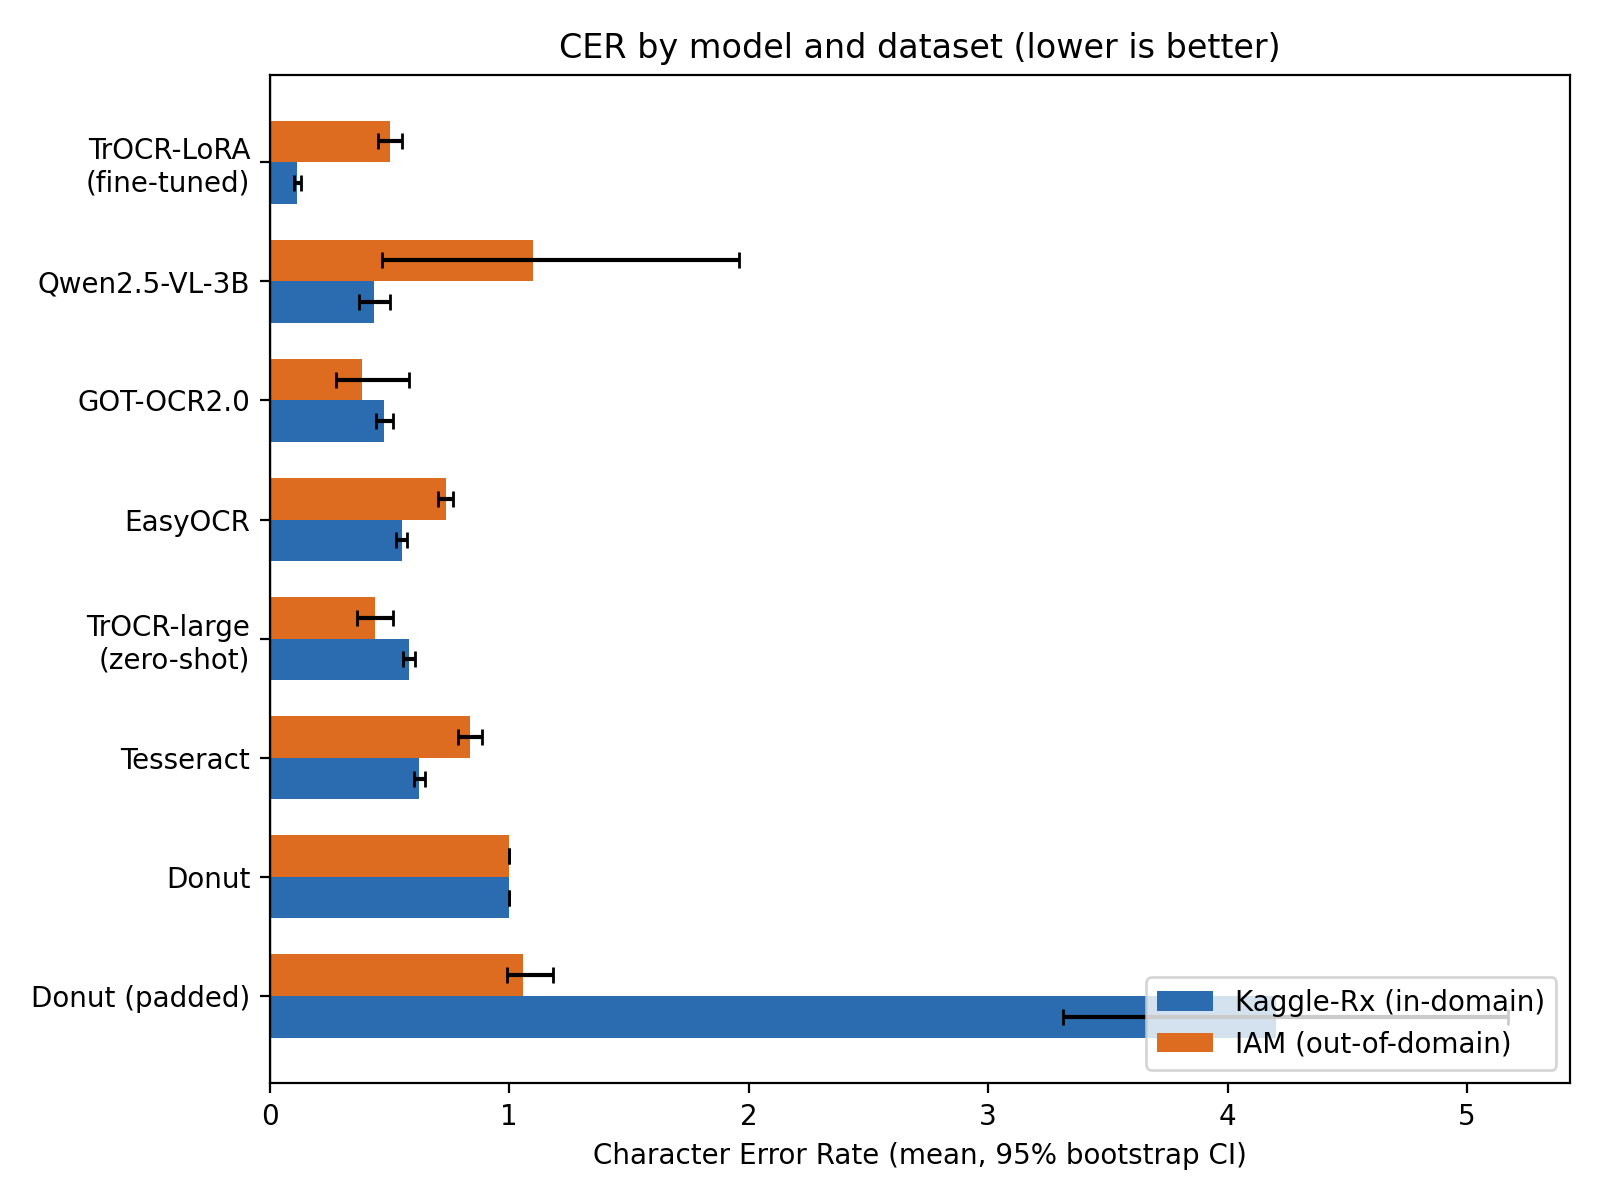
\includegraphics[width=0.85\textwidth]{figures/fig1_cer_comparison.png}
\caption{CER by model and dataset (mean, 95\% bootstrap CI), all eight systems: the seven zero-shot systems
of Table~\ref{tab:zeroshot} plus the fine-tuned model introduced in Section~4.2.}
\label{fig:cer_comparison}
\end{figure}

The strongest zero-shot system on the target, prescription domain is Qwen2.5-VL-3B-Instruct, a
general-purpose 3B-parameter VLM, ahead of every OCR-specialist model we tested, including the
purpose-built GOT-OCR2.0 (roughly 580M parameters; paired Wilcoxon signed-rank, n = 780, Holm-adjusted
$p = 3.8\times10^{-24}$ within the seven-comparison benchmark family; rank-biserial $r_{rb} = -0.49$, a
moderate-to-large effect), as Figure~\ref{fig:cer_comparison} shows alongside the
fine-tuned model introduced in Section~4.2. Taken at face value this is a striking result: a model
with no OCR-specific training objective beats models built specifically to read text, plausibly because
some world knowledge of what a plausible drug name looks like helps it resolve otherwise ambiguous
handwriting. On IAM, GOT-OCR2.0 and TrOCR-large-handwritten --- the latter directly pretrained toward
IAM-like handwriting --- are both strong, while Qwen2.5-VL-3B's \textit{mean} CER (1.100) is the worst of
all seven systems even though its \textit{median} CER is 0.0, meaning more than half its IAM predictions are
exactly right. On inspection, the mean turns out to be driven by a small subset, roughly 3\% of cases, where
the model answers conversationally instead of following the ``output only the text'' instruction --- for
instance, predicting \textit{``The text is not visible in the image provided. Please upload an
image\ldots''} against a one-character ground truth. Against a very short reference, a refusal like that
produces an enormous per-image CER. We read this as two things at once: a substantive finding, that mean
CER can badly mislead when summarizing instruction-tuned VLMs (a paired Wilcoxon test between Qwen2.5-VL-3B
and GOT-OCR2.0 on IAM is \textit{not} significant, $p = 0.330$ --- unchanged after Holm--Bonferroni
correction, since it is already the largest of the seven benchmark-family comparisons; rank-biserial
$r_{rb} = 0.08$, a negligible effect, consistent with the median-driven story below --- despite the large
gap in means), and a
caution for anyone scoring general VLMs as OCR systems using mean error alone. Figure~\ref{fig:cer_dist}
shows this heavy-tailedness directly: several models, Qwen2.5-VL-3B most visibly, have a median CER far
below their mean, with a long tail of high-CER outliers pulling the mean upward.

Donut-base fails almost entirely under both presentations we tried: essentially 100\% degenerate (empty)
output on raw word crops, and, when padded onto a page-sized canvas to better match its pretraining
distribution, a reduced but still high degenerate rate (77.8\% Kaggle-Rx, 96.5\% IAM) accompanied by severe
hallucination on whatever it does produce (mean CER 4.20 and 1.06, respectively). We take this as evidence
that Donut's ``OCR-free,'' full-document pretraining simply does not transfer, absent further fine-tuning,
to isolated single-word recognition --- a useful negative result given how loosely Donut's architecture is
sometimes described as a general-purpose OCR-free document reader.

\begin{figure}[ht]
\centering
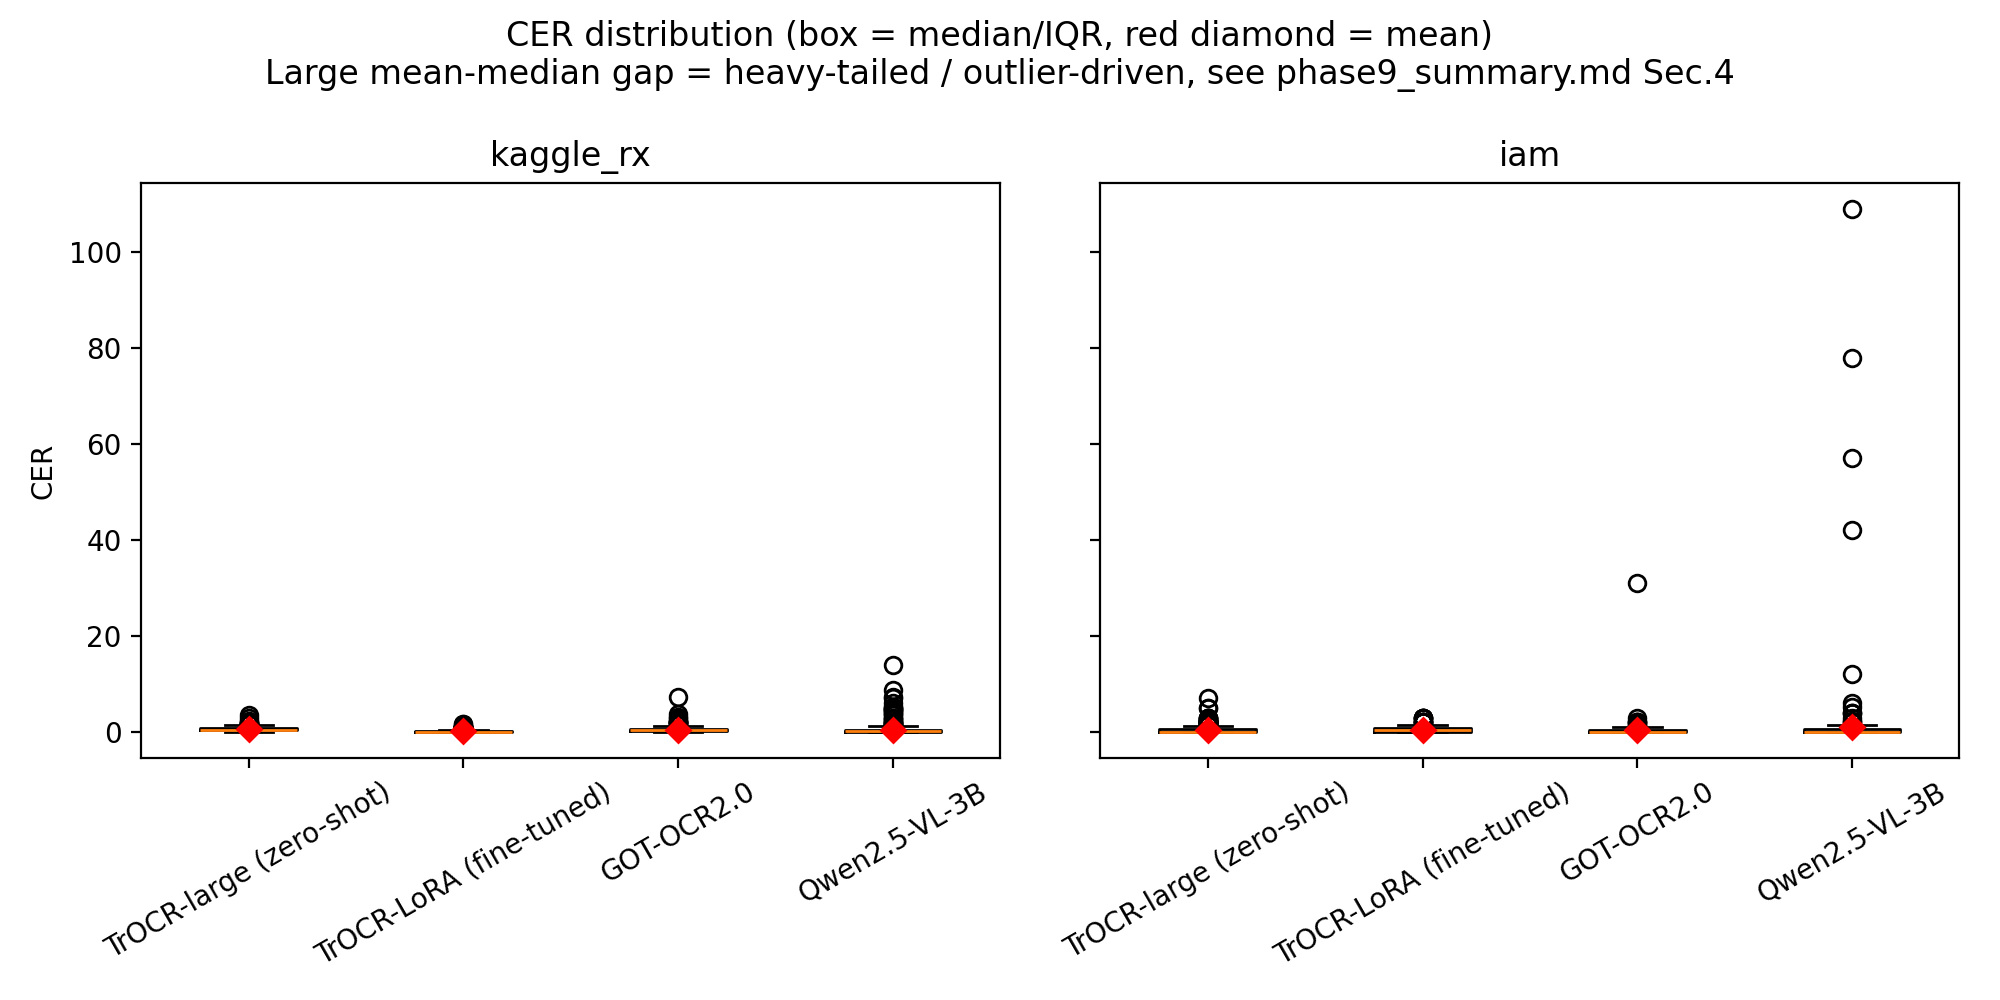
\includegraphics[width=0.85\textwidth]{figures/fig6_cer_distribution.png}
\caption{Per-image CER distributions (box = median/IQR) for the four transformer-based systems, both
datasets. The gap between the box (median) and the mean reported in Table~\ref{tab:zeroshot} is largest for
Qwen2.5-VL-3B on IAM, illustrating the mean/median discrepancy discussed in the text.}
\label{fig:cer_dist}
\end{figure}

\subsection{LoRA fine-tuning and ablation}

\begin{table}[ht]
\centering
\caption{Rank and augmentation ablation on the frozen Kaggle-Rx (n = 780) and IAM (n = 400) test sets. Each
configuration was trained once, to early stopping, on identical data and seed. $p$-values are
Holm--Bonferroni-adjusted within the six-comparison ablation family (Section~3.3); rank-biserial effect
sizes for each comparison are reported in the text.}
\label{tab:ablation}
\small
\begin{tabular}{lccc}
\toprule
Configuration & CER, Kaggle-Rx & CER, IAM & Holm $p$ vs.\ r=16 elastic (Rx / IAM) \\
\midrule
r = 8, elastic & 0.113 [0.098, 0.128] & 0.530 [0.475, 0.580] & $5.0\times10^{-7}$ / $1.00$ \\
r = 16, elastic & 0.149 [0.132, 0.166] & 0.524 [0.472, 0.579] & --- \\
\textbf{r = 32, elastic (selected)} & \textbf{0.114} [0.100, 0.130] & \textbf{0.501} [0.453, 0.552] & $1.4\times10^{-7}$ / $0.32$ \\
r = 16, no elastic & 0.150 [0.134, 0.167] & 0.562 [0.505, 0.627] & $1.00$ / $0.32$ \\
\bottomrule
\end{tabular}
\end{table}

As Table~\ref{tab:ablation} shows, the a priori ``middle'' choice, r = 16, turns out to be beaten on
Kaggle-Rx by both r = 8 and r = 32, and both differences survive Holm--Bonferroni correction within the
six-comparison ablation family: r = 8 (Holm-adjusted $p = 5.0\times10^{-7}$, rank-biserial $r_{rb} = -0.41$)
and r = 32 (Holm-adjusted $p = 1.4\times10^{-7}$, $r_{rb} = -0.47$), both moderate-to-large effects, with the
negative sign reflecting that the non-default rank has the lower, better CER. Neither rank's IAM comparison
with r = 16 survives correction (r = 8: Holm-adjusted $p = 1.00$, $r_{rb} = 0.02$; r = 32: see below), both
negligible effects. r = 32 additionally posts the
best point estimate on IAM, but we want to be explicit that this particular comparison does not survive
correction: the raw $p$-value (0.079) looked close to the conventional 0.05 threshold, but after
Holm--Bonferroni correction within the same six-comparison family it rises to $p = 0.32$, with a small
effect size ($r_{rb} = -0.17$). We therefore treat r = 32's apparent IAM advantage over r = 16 as a favorable
point estimate rather than a statistically established difference, and rely on the two Holm-significant,
in-domain comparisons above --- together with the fact that r = 32 does not underperform r = 16 on IAM in
absolute terms --- to justify using r = 32 as ``the fine-tuned model'' for the rest of this paper. Turning
elastic distortion off, with rank held at 16, leaves in-domain CER essentially unchanged (0.149 versus 0.150;
Holm-adjusted $p = 1.00$, $r_{rb} = 0.04$, a negligible effect) and produces a somewhat worse point estimate
on IAM (0.562 versus 0.524) that likewise does not survive correction (Holm-adjusted $p = 0.32$,
$r_{rb} = 0.15$, a small effect); we kept elastic distortion in the final pipeline because there is no sign
it hurts, and only a small, statistically unconfirmed hint that it helps retention.

Training at r = 32 reaches its best validation CER (0.102 on the 300-image tracking subsample) at epoch~2 of
15, and early stopping triggers at epoch~7 after five epochs without improvement
(Figure~\ref{fig:training_curve}). Validation loss keeps falling past epoch~2 even as validation CER
plateaus and then worsens, which is consistent with the model starting to overfit the small training set on
the loss objective well before that shows up in the CER metric.

\begin{figure}[ht]
\centering
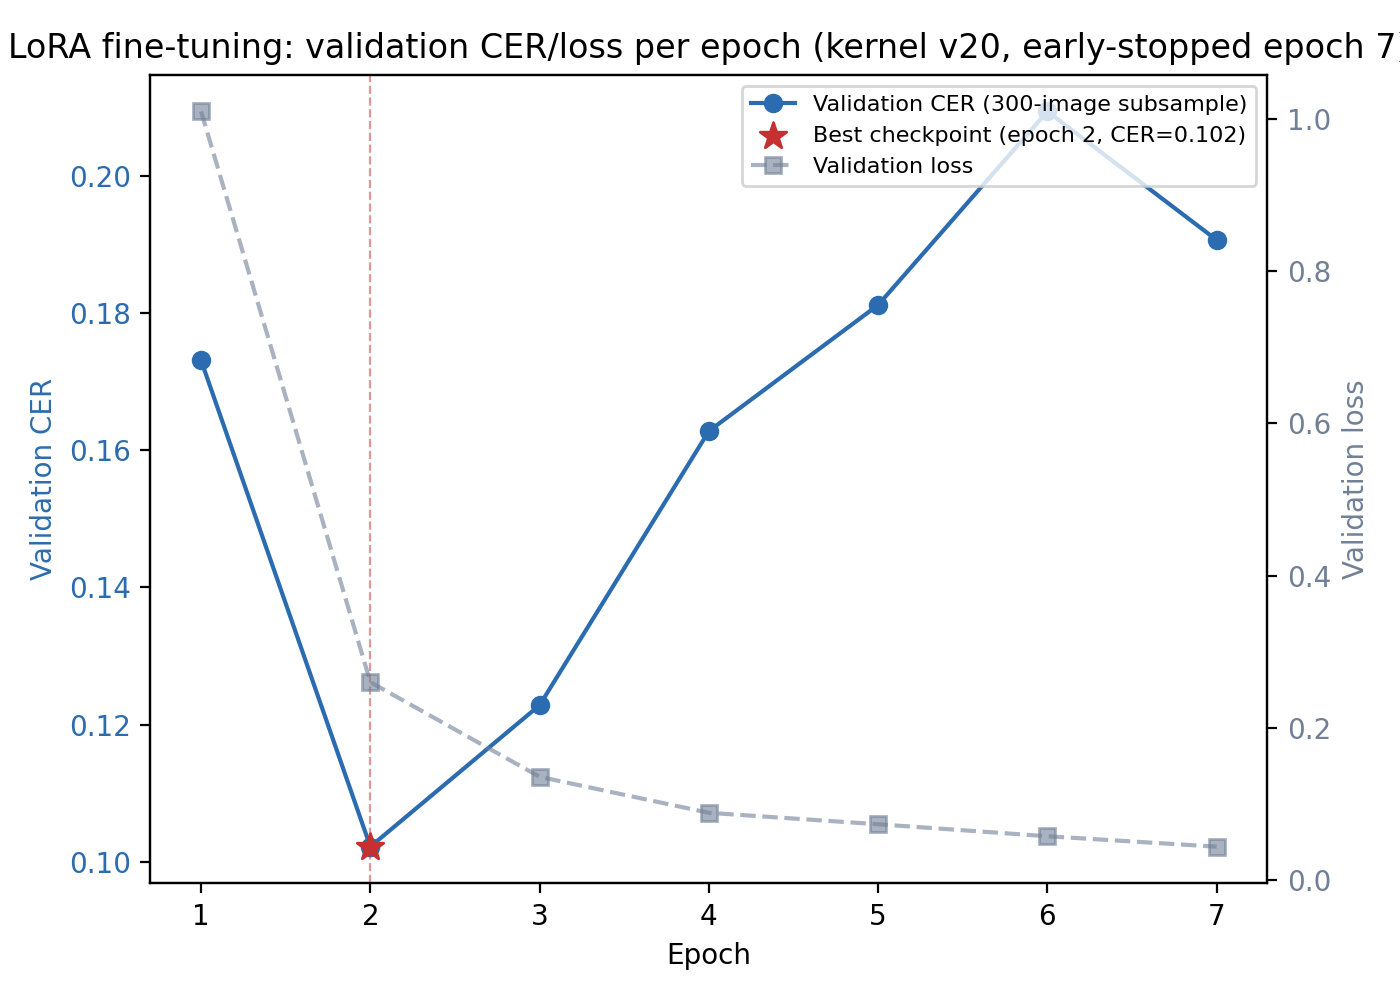
\includegraphics[width=0.75\textwidth]{figures/fig2_training_curve.png}
\caption{LoRA fine-tuning (r = 32): validation CER and loss per epoch, best checkpoint (epoch 2) marked.}
\label{fig:training_curve}
\end{figure}

\subsection{Fine-tuned model versus every zero-shot system}

\begin{table}[ht]
\centering
\caption{Selected model comparison, Kaggle-Rx test set (n = 780).}
\label{tab:headline}
\begin{tabular}{lccc}
\toprule
Model & CER & Exact match & Top-1 acc.\ (78 classes) \\
\midrule
\textbf{TrOCR + LoRA (r = 32, fine-tuned)} & \textbf{0.114} [0.100, 0.130] & \textbf{68.1\%} & \textbf{92.4\%} \\
Qwen2.5-VL-3B-Instruct (zero-shot) & 0.434 [0.372, 0.501] & 28.2\% & 81.5\% \\
GOT-OCR2.0 (zero-shot) & 0.479 [0.446, 0.513] & 15.8\% & 67.2\% \\
TrOCR-large-handwritten (zero-shot) & 0.580 [0.555, 0.606] & 8.1\% & 79.5\% \\
\bottomrule
\end{tabular}
\end{table}

Fine-tuning TrOCR-large-handwritten with LoRA at r = 32, on 3{,}120 images, takes CER from 0.580 zero-shot to
0.114 --- an 80.3\% relative reduction --- and raises exact match from 8.1\% to 68.1\% and closed-vocabulary
top-1 accuracy from 79.5\% to 92.4\% (Table~\ref{tab:headline}). This improvement is itself the largest
paired effect in the paper (Wilcoxon signed-rank, n = 780, Holm-adjusted $p = 4.9\times10^{-110}$ within the
seven-comparison benchmark family; rank-biserial $r_{rb} = 0.97$). The fine-tuned, 558M-parameter model also
beats every zero-shot system we tested on this domain, including systems with far more parameters or
explicit OCR specialization: against Qwen2.5-VL-3B-Instruct (3B parameters), Holm-adjusted
$p = 2.2\times10^{-58}$, $r_{rb} = -0.82$; against GOT-OCR2.0 (roughly 580M parameters, built specifically
for OCR), Holm-adjusted $p = 4.8\times10^{-92}$, $r_{rb} = -0.95$ (paired Wilcoxon signed-rank, n = 780 in
both cases; negative $r_{rb}$ in both comparisons simply because the fine-tuned model attains the lower CER
of the pair). All three effect sizes are large by conventional benchmarks for rank-biserial correlation. As far as
we know, this is the first demonstration that a small, resource-efficient specialist model, adapted with
under 2\% of its parameters on a single free-tier GPU, can decisively outperform much larger general-purpose
VLMs on a target handwriting domain.

\subsection{Domain shift and generalization}

On IAM, the fine-tuned model's CER rises from 0.441 (zero-shot TrOCR) to 0.501 --- a 13.7\% relative
\textit{increase} in error, and a statistically significant one (paired Wilcoxon, n = 400, Holm-adjusted
$p = 6.4\times10^{-4}$ within the seven-comparison benchmark family; rank-biserial $r_{rb} = -0.26$, a
small-to-moderate effect --- noticeably smaller than the $r_{rb} = 0.97$ in-domain improvement above, so we
read this as a real but modest cost, not a comparably large effect in the opposite direction). The median
CER on IAM rises too, from 0.0 zero-shot to 0.400 fine-tuned, which tells us this is a broad, systematic
shift rather than a handful of outlier failures. Figure~\ref{fig:domain_gap} plots the
resulting reversal in domain-shift gap (CER on IAM minus CER on Kaggle-Rx) across every model: zero-shot
OCR-specialist models (TrOCR, GOT-OCR2.0) score slightly \textit{better} on IAM than on Kaggle-Rx, a
negative gap consistent with IAM being closer to their original pretraining distribution than prescription
handwriting is, while the fine-tuned model shows a substantial positive gap --- a direct, quantitative
signature of the specialization it has undergone. The fine-tuned model is also now significantly behind the
strongest zero-shot performer on IAM, GOT-OCR2.0 (0.501 versus 0.386; paired Wilcoxon signed-rank, n = 400,
Holm-adjusted $p = 7.0\times10^{-13}$ within the seven-comparison benchmark family; rank-biserial
$r_{rb} = 0.53$, a moderate-to-large effect), which it was not before fine-tuning specialized it toward
prescription handwriting. One thing worth clarifying so Table~2 is not misread
against this gap figure: the gap being similar in size for r = 16 (+0.376) and r = 32 (+0.387) does not
contradict r = 32 being better on \textit{both} datasets in absolute terms. r = 32 improves Kaggle-Rx
performance by more than it improves IAM performance relative to r = 16, and that is enough to widen the gap
slightly even as both individual numbers get better.

\begin{figure}[ht]
\centering
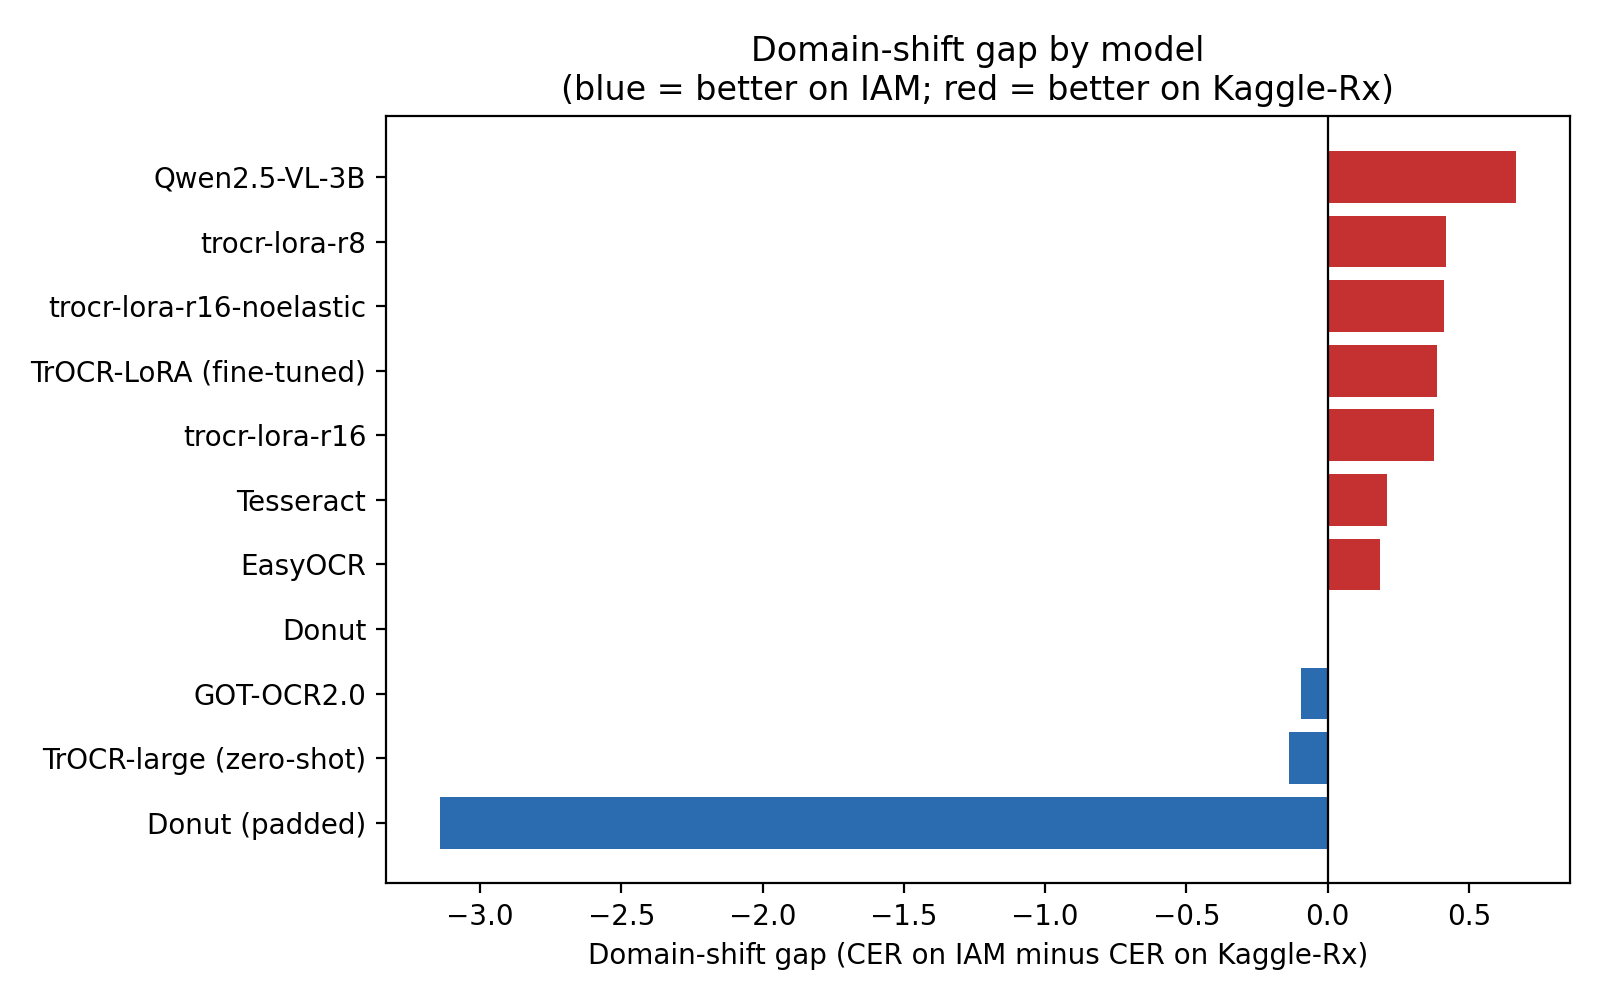
\includegraphics[width=0.75\textwidth]{figures/fig5_domain_gap.png}
\caption{Domain-shift gap (CER on IAM minus CER on Kaggle-Rx) by model. Blue bars score better on IAM; red
bars score better on Kaggle-Rx.}
\label{fig:domain_gap}
\end{figure}

This result sits in some tension with, though does not directly contradict, the claim that LoRA-family
fine-tuning is broadly protective against catastrophic forgetting \citep{Biderman2024LoRALearnsLess}: we did
not run a matched full fine-tuning comparison, so we cannot say LoRA forgets \textit{more} than full
fine-tuning would here, only that updating under 2\% of parameters was not enough, in this setting, to avoid
a statistically significant loss of out-of-domain handwriting ability. That is more consistent with the more
qualified picture in Shuttleworth et al.'s account of LoRA-specific ``intruder
dimensions'' \citep{Shuttleworth2025Illusion} and Kalajdzievski's finding that forgetting under fine-tuning
follows a fairly predictable scaling law rather than being reliably avoided by early stopping
alone \citep{Kalajdzievski2024Scaling}.

\subsection{Qualitative error taxonomy and clinical safety implications}

\begin{table}[ht]
\centering
\caption{Error-category composition, Kaggle-Rx test set, zero-shot vs.\ fine-tuned (r = 32).}
\label{tab:errortax}
\begin{tabular}{lcc}
\toprule
Category & Zero-shot & Fine-tuned \\
\midrule
Correct (exact match) & 8.1\% & 68.1\% \\
Minor OCR noise, still correct drug & 71.8\% & 24.9\% \\
Confusable wrong drug (resembles a \textit{different} real drug) & 1.5\% & 2.6\% \\
Hallucination, far off (resembles no real drug) & 18.6\% & 4.5\% \\
\bottomrule
\end{tabular}
\end{table}

\begin{figure}[ht]
\centering
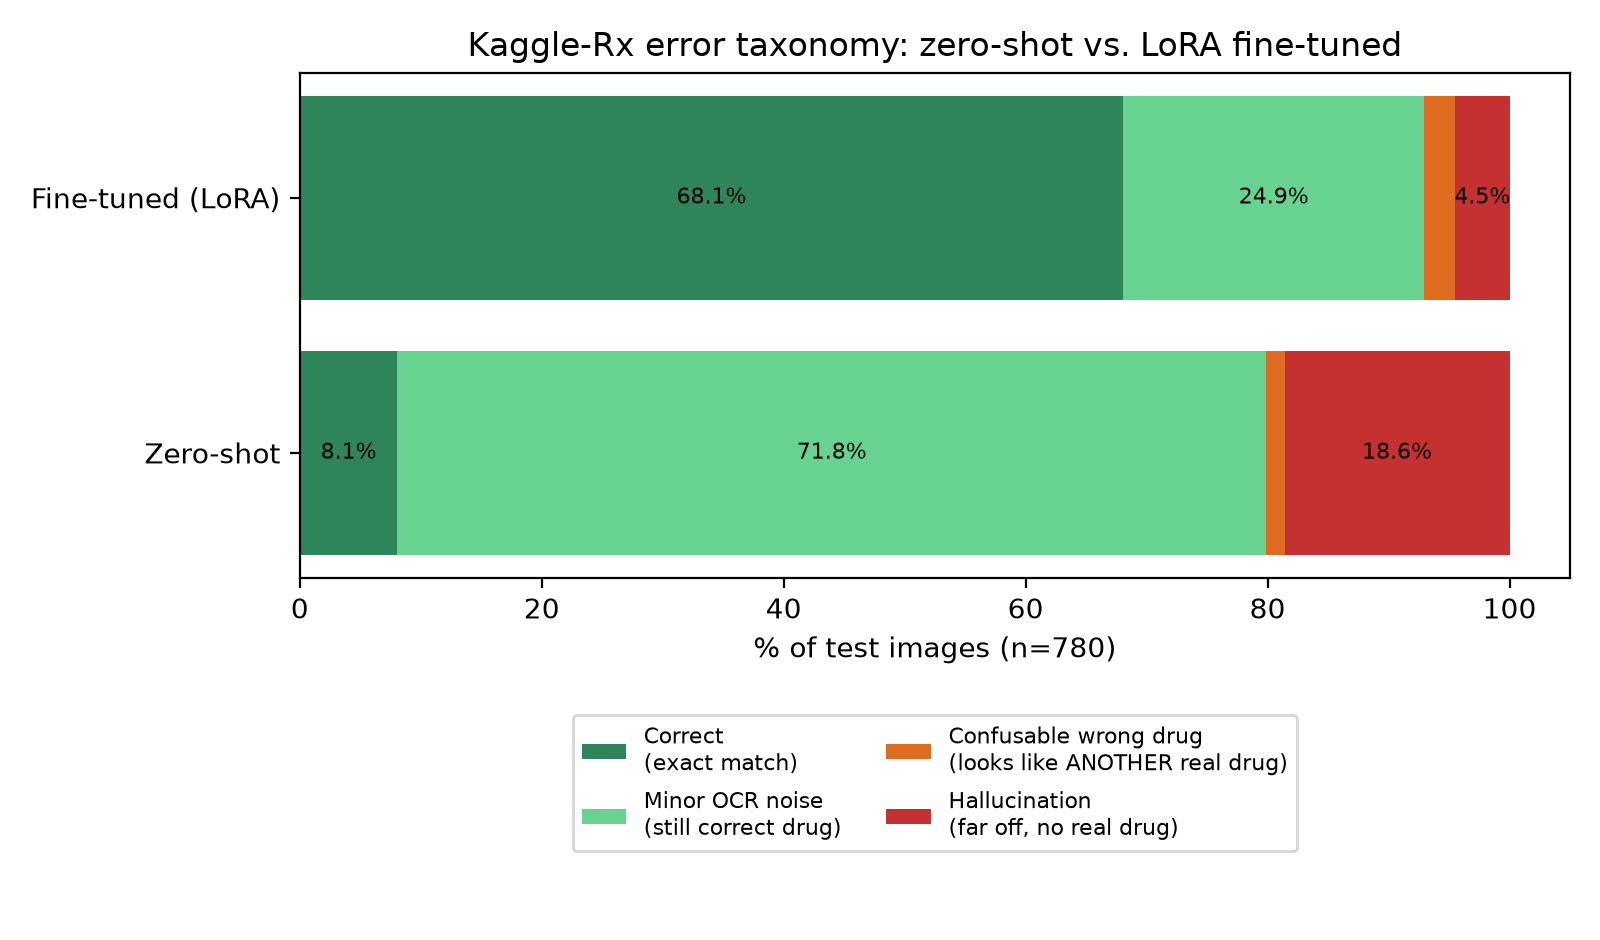
\includegraphics[width=0.8\textwidth]{figures/fig3_error_taxonomy_kaggle_rx.png}
\caption{Kaggle-Rx error-category composition (Table~\ref{tab:errortax}), zero-shot vs.\ fine-tuned.}
\label{fig:errortax_rx}
\end{figure}

Fine-tuning cuts the outright-nonsensical ``hallucination, far off'' category roughly fourfold (18.6\% to
4.5\%): the model becomes much less prone to guessing wildly. But the smaller category of errors that
resemble a \textit{different, real} drug name rises from 1.5\% to 2.6\%, a 1.7-fold relative increase. We
think this is the most clinically relevant result in the paper. A prediction that reads as \textit{some
other real medicine} --- for instance, ground truth ``Amodis'' misread as ``Amodin,'' which itself sits
closer to the unrelated real drug ``Axodin'' than to the correct answer (Figure~\ref{fig:qualitative} shows
this and three other examples) --- looks plausible on its face and,
by the look-alike/sound-alike medication-error
literature \citep{Bryan2021LASA,Ostini2012LASA,Karet2023TallMan}, is considerably harder to catch on routine
manual review than output that plainly is not a real drug name. Aggregate CER improves a great deal under
fine-tuning, but the \textit{composition} of what error remains shifts toward the category that is arguably
most dangerous in a deployed system, a distinction that CER alone cannot see. We also checked one further,
more specific risk: whether the fine-tuned model, having been narrowly specialized on 78 drug names, starts
inserting a memorized drug name when reading unrelated general handwriting. Of 400 IAM predictions, only
2 (0.5\%, versus 0 of 400 for the zero-shot model) exactly matched a Kaggle-Rx drug name while being clearly
wrong relative to the true IAM label; both are plausibly chance collisions on a short or difficult word
rather than systematic drug-name intrusion, and we do not think this rises to a meaningful effect at our
sample size.

\begin{figure}[ht]
\centering
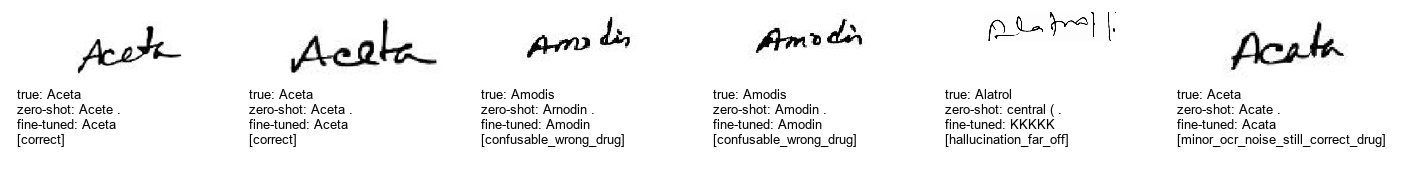
\includegraphics[width=0.95\textwidth]{figures/fig7_qualitative_examples.png}
\caption{Representative Kaggle-Rx word crops with ground truth, zero-shot, and fine-tuned predictions, one
example per error category from Table~\ref{tab:errortax} (left to right: correct $\times2$, confusable
wrong drug $\times2$, hallucination, minor OCR noise).}
\label{fig:qualitative}
\end{figure}

On IAM, the error-severity distribution moves from 57.3\% exact match / 12.8\% moderate error / 23.3\%
severe error zero-shot to 26.8\% / 32.8\% / 27.5\% fine-tuned (Figure~\ref{fig:errortax_iam}) --- mostly a
shift from exactly correct to moderately wrong, rather than toward outright failure, which adds some nuance
to the mean/median framing of Section~4.4: fine-tuning on a narrow domain degrades a broad swath of
previously perfect out-of-domain predictions to ``partially wrong'' more than it manufactures new
catastrophic failures.

\begin{figure}[ht]
\centering
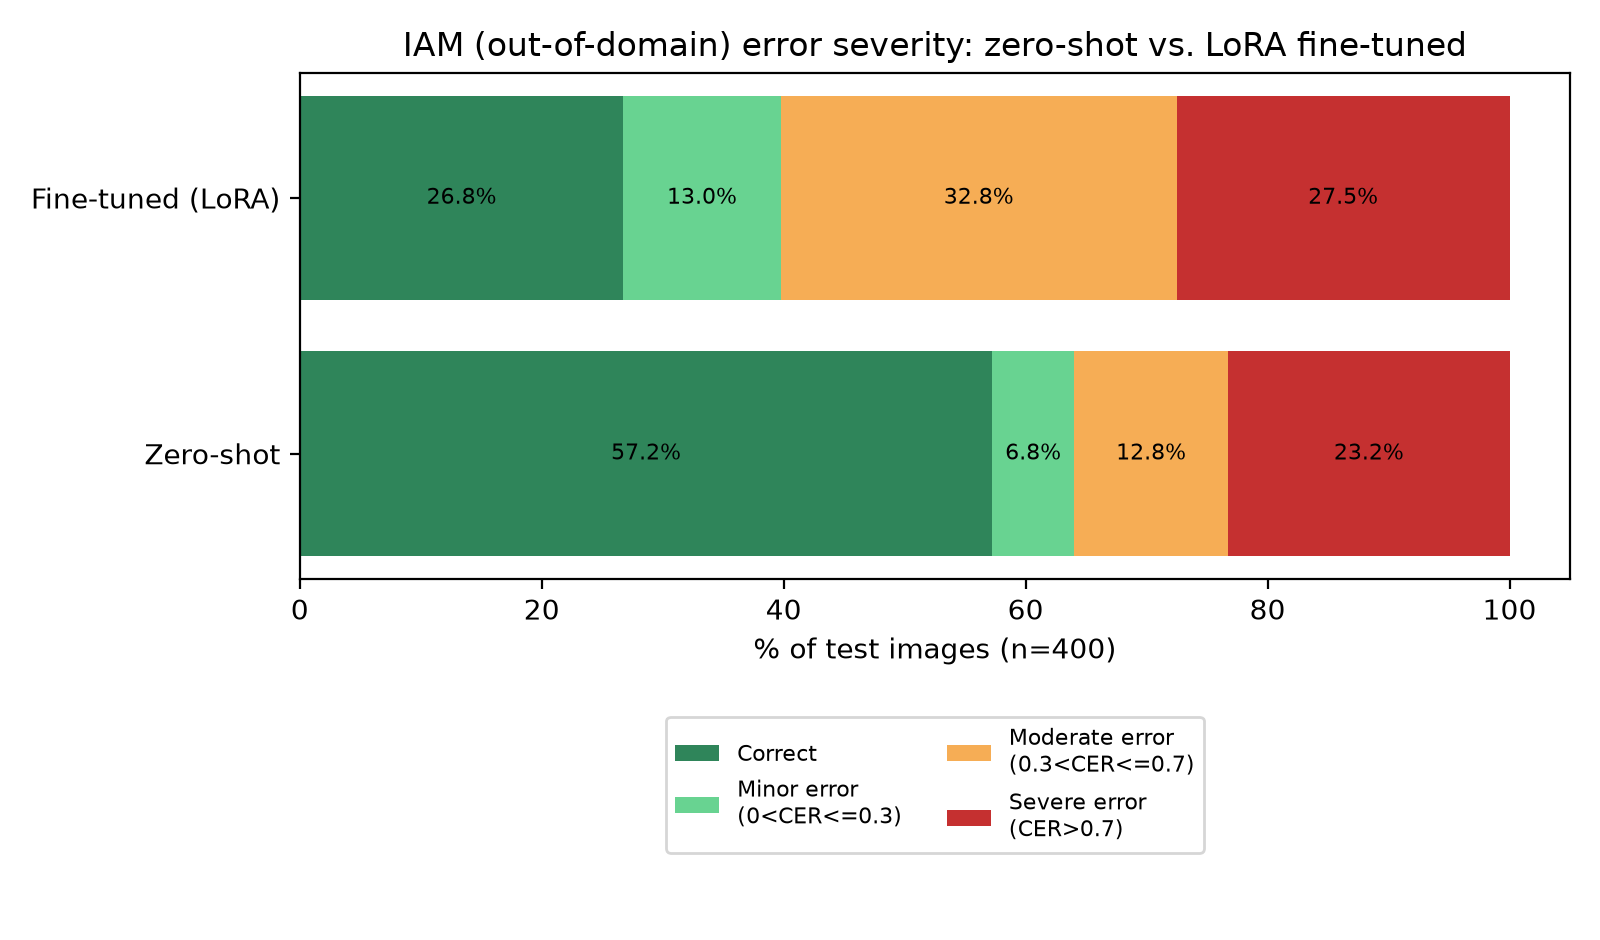
\includegraphics[width=0.8\textwidth]{figures/fig4_error_taxonomy_iam.png}
\caption{IAM error-severity composition, zero-shot vs.\ fine-tuned.}
\label{fig:errortax_iam}
\end{figure}

\section{Discussion}

\textbf{A small, cheaply adapted specialist can beat much larger general VLMs on a target domain.} The
headline result here --- that LoRA-adapting a 558M-parameter model on a single free-tier GPU, touching
under 2\% of its parameters, produces a decisive improvement over a 3B-parameter general VLM and a
purpose-built 580M-parameter OCR model --- matters beyond the specific numbers. For teams without large
compute budgets, which describes most low- and middle-income-country health-informatics groups and,
frankly, the independent and self-funded circumstances of this study, fine-tuning a small specialist model
on a modest, domain-relevant dataset is both more accessible and more effective than leaning on ever-larger
general-purpose models zero-shot.

\textbf{Rank matters, and a reasonable-sounding default is not a substitute for checking.} A LoRA rank of 16
is a common default in the fine-tuning literature, and it was our own initial plan. Our ablation shows that,
in this setting, it was beaten by both a smaller rank (8) and a larger one (32) on the in-domain metric, with
no compensating advantage on generalization. We flag this mainly as a methodological caution: without the
ablation, we would have reported a materially weaker headline result (CER 0.149 rather than 0.114) under the
mistaken impression that it was close to optimal.

\textbf{LoRA does not eliminate catastrophic forgetting here.} The Section~4.4 result --- a statistically
significant, systematic degradation on out-of-domain handwriting after updating under 2\% of parameters ---
sits uneasily next to the idea that PEFT methods are largely protective against
forgetting \citep{Biderman2024LoRALearnsLess}, though it does not contradict that work directly, since we
never ran a matched full fine-tuning comparison. It fits more comfortably with the more qualified account in
Shuttleworth et al.'s ``intruder dimensions'' \citep{Shuttleworth2025Illusion}. Practically, this
suggests that anyone fine-tuning a general HTR model for a narrow domain should budget for an
out-of-domain check, rather than assuming a small trainable-parameter fraction is protection enough on its
own.

\textbf{Error type, not just error rate, determines clinical risk.} The Section~4.5 finding --- that
fine-tuning improves aggregate accuracy while shifting the residual-error mix toward outputs that resemble a
different real medication --- is, as far as we can tell, the first result connecting this specific
mechanism to medication-name-confusion safety risk in an OCR setting. The broader principle that error
\textit{type} matters more than error \textit{rate} for clinical risk has precedent in
speech-recognition-assisted clinical documentation \citep{Zhou2018JAMA}, and the LASA
literature \citep{Bryan2021LASA,Ostini2012LASA,Karet2023TallMan} independently establishes that
confusable-real-drug-name errors are a recognized, clinically significant category on their own; our
contribution is tying these together with a concrete, measured shift under a common OCR fine-tuning
intervention. In practice, this argues for evaluating and, ideally, optimizing prescription-OCR systems
against a confusable-drug-aware metric rather than aggregate CER alone, and for a lexicon- or
LASA-list-aware post-processing correction stage as a natural next step, which we did not implement here
(Section~7).

\textbf{Reproducibility lessons for the OCR/VLM community.} Two of the seven systems we set out to
benchmark needed real debugging before they produced valid output, and one, PaddleOCR-VL, could not be run
to completion at all. GOT-OCR2.0 produced fluent-looking but essentially random multilingual output under
an unpinned, newly released major \texttt{transformers} version, and was only fixed by pinning to an earlier
release; PaddleOCR-VL raises an unresolved \texttt{trust\_remote\_code} incompatibility under every
\texttt{transformers} version we tried, matching an open, unresolved community bug report at the time of
writing. We record these not as incidental engineering footnotes but as a substantive observation: models
released and updated outside a library's core, stable release cadence carry a real, non-obvious
reproducibility cost for downstream benchmarking that is separate from how good the underlying model
actually is.

\section{Limitations}

\begin{itemize}[leftmargin=*]
\item \textbf{One training dataset per domain.} We use a single public prescription dataset, with its own
particular 78-drug vocabulary and handwriting population, and a single general-handwriting control (IAM).
Results may not carry over to prescription handwriting in other languages, health systems, or drug-name
vocabularies.
\item \textbf{One random seed per fine-tuning configuration.} Each of the four ablation configurations
(Sections~3.4, 4.2) was trained exactly once. The paired Wilcoxon tests tell us the specific trained
checkpoints differ significantly on the frozen test sets; they do not tell us that repeated training runs at
a given rank would reliably reproduce the same ranking, and part of the observed rank effect could be
run-to-run training variance. A replication with at least five independent training seeds per rank,
reporting mean $\pm$ SD CER/WER and re-running the same Wilcoxon signed-rank plus Holm--Bonferroni plus
rank-biserial pipeline (Section~3.3) across seeds, would be needed to establish whether the r = 8/32-over-16
ordering reflects a true rank effect rather than seed noise; we did not have the compute budget for this
within the free-tier GPU constraints of the study.
\item \textbf{PaddleOCR-VL could not be benchmarked}, owing to an unresolved upstream library
incompatibility, leaving one of the four general-VLM systems we set out to test excluded from quantitative
comparison.
\item \textbf{A small, closed-vocabulary fine-tuning target.} The 3{,}120-image training set and 78-class
label space mean some of the fine-tuned model's strong in-domain performance is attributable to a genuinely
narrow task. We do not evaluate performance on drug names outside this 78-class vocabulary, or on
dosage/frequency text beyond the drug name itself.
\item \textbf{The 0.34 confusable-drug distance threshold (Section~3.5) is a design choice, not a
clinically validated cutoff.} We report it transparently; a formal LASA-pair-based definition, following
Karet \citep{Karet2023TallMan}, would be a natural refinement.
\item \textbf{IAM is one particular operationalization of ``general handwriting.''} Generalization loss
measured against IAM may not represent generalization loss against other out-of-domain distributions:
other languages, other prescription vocabularies, or clinical free text.
\item \textbf{No clinician or pharmacist review.} Our safety-relevant error-taxonomy claims rest on
automated, distance-based categorization and the published LASA literature, not on a clinical expert's
review of the specific errors observed. We see such a review as a valuable next step, not a substitute for
the quantitative analysis reported here.
\end{itemize}

\section{Conclusion}

We benchmarked seven OCR and vision-language systems, zero-shot, on a public handwritten medical
prescription dataset and an out-of-domain handwriting control, and found that a general-purpose
3B-parameter VLM outperforms every OCR-specialist system on the target domain. We then showed that
lightweight LoRA fine-tuning of a much smaller, 558M-parameter specialist model, using under 2\% of
trainable parameters on a single free-tier GPU, statistically outperforms every zero-shot system tested,
after a rank and augmentation ablation that overturned our own initial choice of hyperparameter. That
improvement comes with a statistically significant, though partial, loss of general handwriting ability,
and, more subtly, with a shift in the composition of the errors that remain toward outputs resembling a
different real medication, a category we argue is more clinically dangerous than obviously wrong output
despite not showing up as a problem in aggregate error-rate terms. Future work could evaluate a lexicon- or
LASA-list-aware post-correction stage aimed at this specific error category, test whether mixing a small
amount of general-handwriting data into fine-tuning reduces the observed forgetting without giving up
in-domain gains, and extend this benchmark to further public prescription datasets and languages as they
become available.

\section*{Additional Information}

\paragraph{Data availability.} All code (benchmark pipeline, fine-tuning script, analysis scripts, figure
generation), the frozen evaluation manifests, per-image predictions for every model, and the final LoRA
adapter weights are available at \textbf{[repository URL --- to be added]}. Both datasets are public: Kaggle-Rx
at \url{https://www.kaggle.com/datasets/mamun1113/doctors-handwritten-prescription-bd-dataset}, and IAM
through its standard registration process at \url{https://fki.tic.heia-fr.ch/databases/iam-handwriting-database};
readers
should independently check the exact license terms on each dataset's page before redistributing it.

\paragraph{AI-use disclosure.} The author used Claude (Anthropic), accessed via Claude Code,
throughout this project's development (15--18 September 2026) to assist with drafting and editing manuscript
prose, writing and reviewing the statistical-analysis code described in Section~3.3
(\texttt{src/analyze\_\allowbreak statistics.py}), generating the figures in Section~4, and literature
search and citation triage. Specifically: Claude Sonnet 5 (model ID claude-sonnet-5) produced the majority of
the code commits, the LaTeX manuscript draft, the statistical-reporting script, and the final editing pass
reported here (17--18 September 2026); Claude Haiku 4.5 (model ID claude-haiku-4-5-20251001) was
used for portions of manuscript review and venue-verification research on 18 September 2026. % TODO(author):
% the earlier development sessions (15--16 September 2026) that produced the benchmark and fine-tuning
% pipeline predate this project's practice of recording model identity in commit metadata, so the exact
% Claude model version(s) used in those specific sessions could not be reconstructed from the available
% record and are omitted here rather than guessed at -- please confirm and add if you recall which model(s)
% you used in that earlier period, or leave as-is if unconcerned.
The author (B.\,Dang) directed all research decisions, designed and ran every experiment,
independently verified every statistic, figure, and citation reported in this manuscript, and takes full
responsibility for its content. No generative AI tool is listed as an author, and no AI tool was used to
create, alter, or fabricate any research image or experimental data.

\paragraph{Funding.} This work received no external funding; compute was provided by Kaggle's free-tier GPU
quota.

\paragraph{Competing interests.} The author declares no competing interests.

\paragraph{Author contributions.} B.D. conceived the study, designed and ran all experiments, performed
the analysis, and wrote the manuscript.

\bibliographystyle{plainnat}
\bibliography{references}

\end{document}
